\chapter{Tools} 
Multiple tools were used in the process of creating the demo application for
this paper including the Unity game engine, Blender as a modeling and animation
software, and MakeHuman as a model creation tool. This chapter discusses the
built-in functionalities which make the mentioned tools an effective choice.

\section{MakeHuman}
MakeHuman is an open source tool for making 3D characters. It provides
a convenient way of acquiring a human model which is customizable and can be
exported in various formats in order to be used in other software programs. The
key factors which make this tool suitable for use in the demo application is the
options it provides regarding the complexity of the topology of the model's
mesh, and the choice of skeleton rig alongside the fact that the exported model
is already rigged and ready to be used in an animation software. One of the rig
presets, which is shown in Fig. \ref{fig:mh_rig}, is specifically designed to be
used for video games.

\begin{figure}
    \centering
    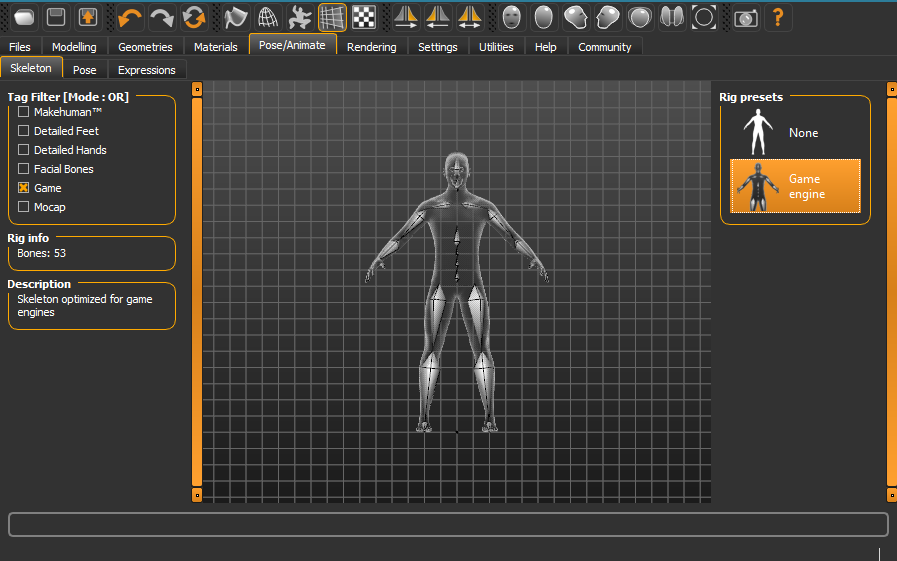
\includegraphics[width=\textwidth]{grafika/make_human_rig.png}
    \caption{MakeHuman rig selection}
    \label{fig:mh_rig}
\end{figure}

\section{Blender}
The tool of choice for modeling and animation used for the demo application is
Blender. It is a free and open source tool offering a suite of functionalities
including the creation of 3D models, rigging, and animation. 

% The program enables
% users to import models in various formats, which allows the user to use
% externally generated models, such as the ones created in MakeHuman, and animate
% them. 

Blender offers the functionality of importing existing models in various formats
including the \textit{collada} format \cite{collada} which is the default export
option in MakeHuman. Models can also be created from scratch. Blender offers
a 3D modelling tool to create a desired mesh. A custom rig can also be
constructed and attached to the created model. Weights can be painted on the
mesh's vertices for each bone, to define how tightly they are bound, and how
much the position of each vertex depends on the given bone position. 

Lastly, an animation sequence can be created for an existing mesh and rig using
the character animation pose editor. The user can define poses for different
points in time by creating key frames on a timeline, and blender interpolates the
bone positions in between the key frames. This is used to create baked animations
for characters and objects, as well as defining animations that are later
blended with IK procedural animations. An animated model can be exported in the
\textit{fbx} format to be used in other software programs. Unity also supports
importing a model from a \textit{.blend} file which is the extension of
a blender project file. 


\section{Unity}
The Unity game engine is the one tool which was non-negotiable as the paper
is meant to specifically focus on the usage of inverse kinematics in said game
engine. Nevertheless, the engine is a good selection for this use case due to
its advanced 3D support, the built-in packages and functionalities which are
geared towards the subject of this paper, and the overall popularity of the
engine and large community built around it which results in a substantial amount
of documentation and support. 

\subsection{Importing Animations}
Unity enables users to import animated models from external sources using an
\textit{FBX} file or by importing project files from 3D modeling and animation
software such as Blender, Autodesk Maya, Cinema4D, or Autodesk 3ds Max
\cite{unity_import}. However, the modeling software must be installed on the
user's machine in order to import a model from project files, as Unity uses the
programs themselves to unpack the file. 

When importing an animated model into Unity, the import settings allow the user
to break the animation into multiple parts based on start and end times (Figure
\ref{fig:anim_chunk}). This is convenient, as it allows multiple animations made
in Blender to be placed on a timeline one after the other as a single
animation, which can then be broken up in Unity. It also allows the user to
extract multiple different variations of the same animation, such as importing
the full animation as one whole chunk and also breaking it up into separate
animations for different use cases.

\begin{figure}
    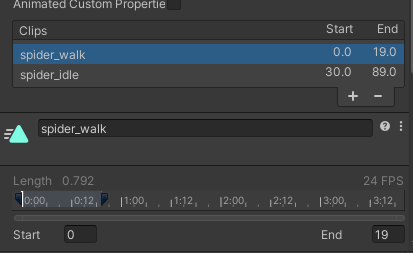
\includegraphics[width=0.5\textwidth]{grafika/animation_chunk_1.png}
    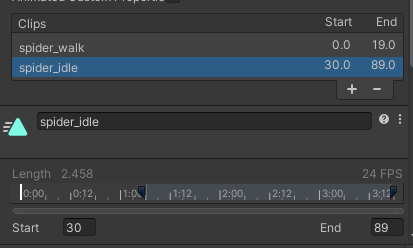
\includegraphics[width=0.5\textwidth]{grafika/animation_chunk_2.png}
    \caption{Animation clips extracted from a single animation during import}
    \label{fig:anim_chunk}
\end{figure}

\subsection{Animator Controller}
An Animator controller allows the user to maintain a set of animation clips, and
the associated transitions which control the flow between each clip in the form of
a state machine (Figure \ref{fig:anim_state}). Animations must be added to an
Animator controller in order to be used by a Unity \textit{GameObject}
\cite{unity_animator}. States can also be controlled procedurally from scripts
by accessing an Animator component which must be attached to the Unity
\textit{GameObject} and must hold a reference to the given Animator controller.
 
\begin{figure}
    \centering
    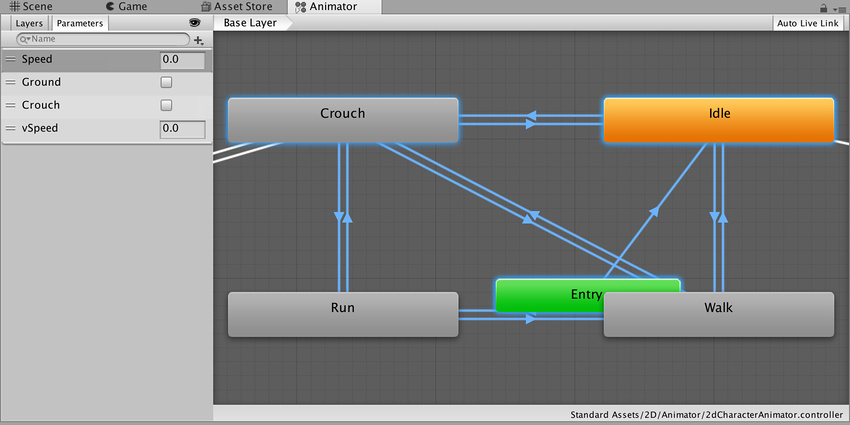
\includegraphics[width=\textwidth]{grafika/animator_controller.png}
    \caption{Animator controller animation state machine \cite{unity_animator}}
    \label{fig:anim_state}
\end{figure}

The Animator controller also has built in IK functionality. This is only
available for humanoid models which have a correctly configured avatar
\cite{unity_ik}. A humanoid avatar is available for models which adhere to a set
of defined general guidelines. In essence, a model which falls into the humanoid
category must have at least 15 bones which are organized in a way which
resembles a human skeleton \cite{unity_humanoid_import}. Humanoid characters
have a few additional functionalities. Namely, because of the criteria required
to qualify as a humanoid model, these models are all similar in structure and as
such, animations can be mapped from one humanoid model to another
\cite{unity_humanoid_avatars}. Additionally, these model's have built in
functionality which allows the developer to procedurally control the models IK
weights and positions using the \textit{SetIKPositionWeight,
SetIKRotationWeight, SetIKPosition, SetIKRotation, SetLookAtPosition,
bodyPosition, bodyRotation} functions \cite{unity_ik, unity_humanoid_avatars}.
Because these methods aren't available to skeletal structures which do not fit
the humanoid description, they are not applicable to the demo application
created for this paper.

\subsection{Animation Rigging Package}

The Animation Rigging package is available in the Unity Package Manager, and it
provides a much more general approach to the application of inverse kinematics
to skeletal animations. After setting up a rig for a model with an Animator
component, a mix of predefined constraints can be added to enhance the rig
(Figure \ref{fig:ar_constraints}). The main constraint of interest for this
paper is the \textit{Chain IK Constraint} which implements the FABRIK algorithm.
This constraint was useful in creating a proof of concept for the spider before
creating the FABRIK script. It also provided a good basis for the public
interface which such a script should have to function well in the Unity
environment.

\begin{figure}
    \centering
    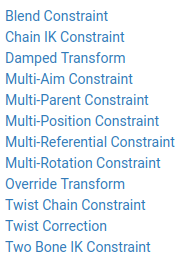
\includegraphics[width=0.3\textwidth]{grafika/ar_constraints.png}
    \caption{Predefined rig constraints available in Unity's Animation Rigging
    package \cite{ar_constraints}}
    \label{fig:ar_constraints}
\end{figure}

